\section{Mastodon numerical features.}
\label{FeaturesExplanation}

This chapter describes how the feature values currently available in Mastodon are calculated. 
We also gives information about their dimension, units, \etc.

\subsection{Feature dimensions.}

In Mastodon, feature values are expressed when possible in physical units. 
Each feature projection as a \textit{dimension} (in the physics meaning) from which we compute the \textit{units} of the values.
For instance, if a feature value as the dimension \texttt{LENGTH} and the spatial units is µm, then the values of this feature will be in~µm.
Mastodon only has physical units for space. 
For time, the frame interval is always equal to the dummy \texttt{1~frame}.
This is why you will find all units involving time expressed in \texttt{frame}s.
Each feature projection has a dimension, and the features report what are the dimension of their projections in the feature computation dialog (Figure~\ref{fig:FindFeatureDimension}).
Here is the table of all the feature dimensions currently supported in Mastodon, and example of the derived units when the spatial units are~µm.

\begin{figure}
    \centering
    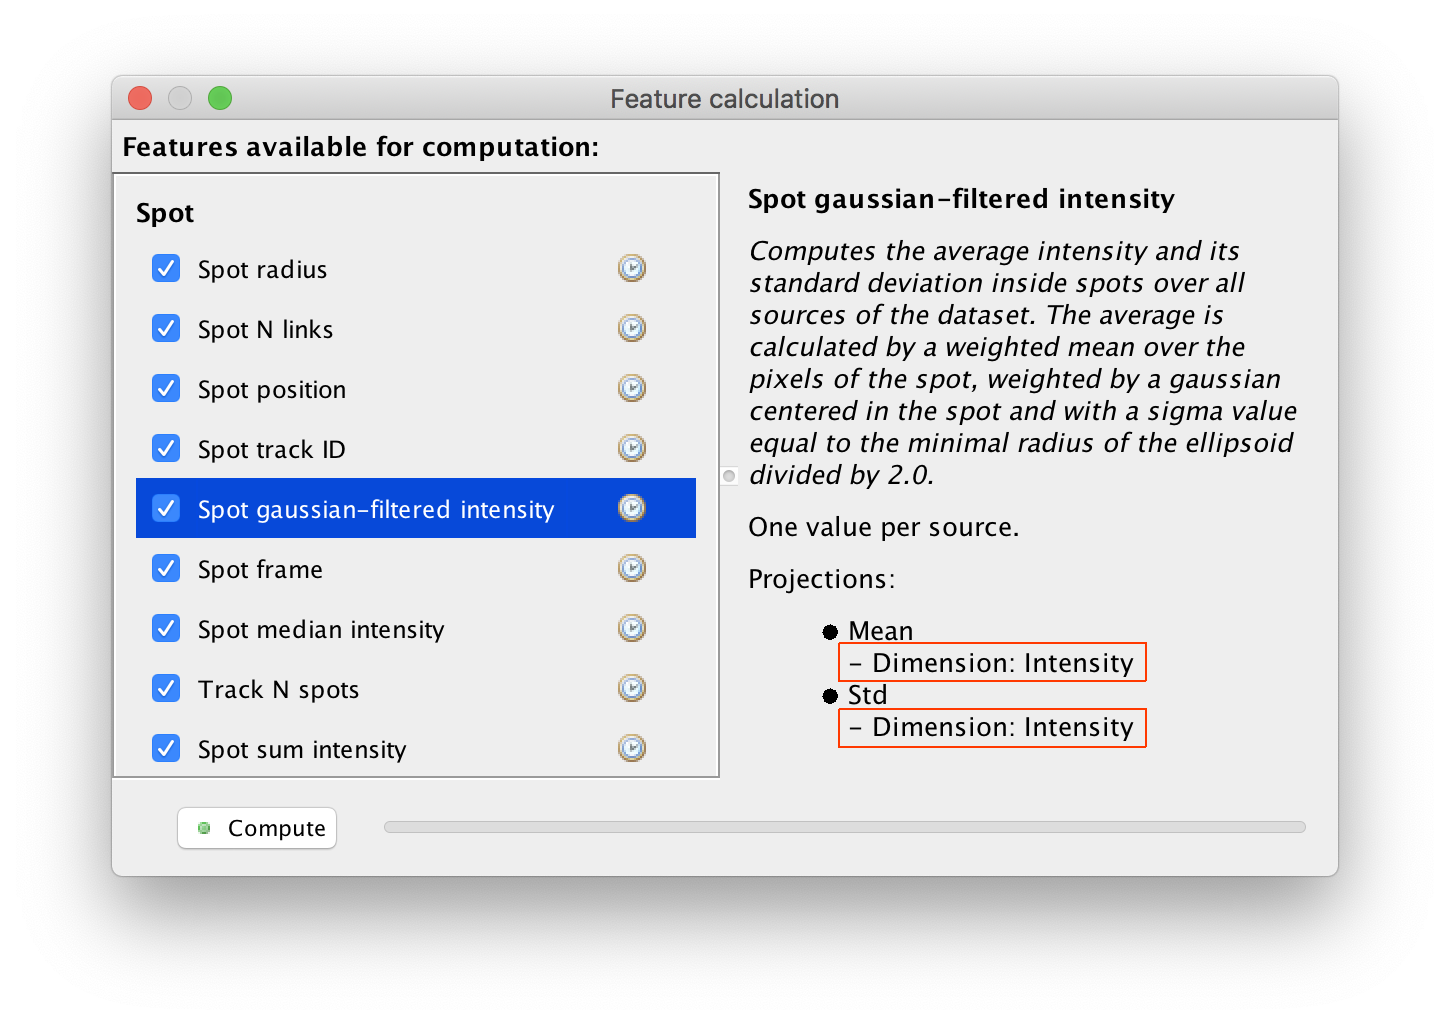
\includegraphics[width=0.4\textwidth]{figures/Mastodon_FindFeatureDimension.png}
    \caption{The feature dimensions are listed in the feature computation dialog, in the description panel that appears on the right when you click on a feature name.}
    \label{fig:FindFeatureDimension}
\end{figure}

\begin{table}
    \centering
    \footnotesize
    \begin{tabular}{ l | l | p{0.125\textwidth} | p{0.50\textwidth} }

    \toprule
    \textbf{Dimension} &
    \textbf{Name} &
    \textbf{Example units (when spatial units are µm)} &
    \textbf{Description}
    
    \\ \midrule
    
    \texttt{NONE} &
    None &
    ø &
    Used for dimensionless quantities, such as frame position, number of things, \etc 
    \\ \midrule
    
    \texttt{LENGTH} & 
    Length &
    µm &
    For quantities about the length of objects. 
    For instance radius or distance between objects.
    \\ \midrule
    
    \texttt{POSITION} & 
    Position &
    µm &
    Dimension for feature that report a position.
    Different from \texttt{LENGTH} so that for objects with small lengths at large positions, quantities are plotted separately.
    \\ \midrule
    
    \texttt{TIME} &
    Time &
    frame &
    For quantities that report a delay, a duration or the timing of an event.
    Because Mastodon does not deal with physical units for time, quantities formed with the time dimension always use the \texttt{frame} unit.
    \\ \midrule
    
    \texttt{VELOCITY} & 
    Velocity & 
    µm / frame &
    For quantities that report a speed or a velocity.
    \\ \midrule
    
    \texttt{RATE} &
    Rate &
    / frame &
    For quantities that report a change per units of time.
    \\ \midrule
    
    \texttt{ANGLE} &
    Angle &
    Radians &
    Measures of angles. 
    In Mastodon, all angles are in \textbf{radians}.
    \\ \midrule
    
    \texttt{STRING} &
    NA &
    ø &
    For non-numeric features.
    \\ \midrule
    
    \texttt{INTENSITY} &
    Intensity &
    Counts &
    For quantities based on pixel values.
    For instance the mean intensity within a spot.
    \\ \midrule
    
    \texttt{INTENSITY\_SQUARED} &
    Intensity² &
    Counts² &
    For quantities based on pixel intensity squared.
    For instance the variance of the mean within a spot.
    \\ \midrule
    
    \texttt{QUALITY} &
    Quality &
    ø &
    This dimension is used by spot detectors.
    There is a special feature called \textbf{Detection quality}, that stores for each spot they detect automatically a measure of quality or confidence in their detection.
    See section~\ref{Detection_Cells_DoG_Detector}.
    \\ \midrule
    
    \texttt{COST} &
    Cost &
    ø &
    This dimension is used by spot linking algorithms.
    There is a special feature called \textbf{Link cost} used in the estimation phase.
    It stores for each link the cost that the linker computes for it in the estimation phase.
    These costs are then used in the association phase to retrieve the best set of links.
    \\ \bottomrule

\end{tabular}
    \caption{Feature dimensions in Mastodon.}
    \label{tab:FeatureDimensions}
\end{table}

\subsection{Spot features.}

\subsubsection{Spot gaussian-filtered intensity.}

This feature has two projections per channel, \textbf{Mean} and \textbf{Std}.
The values are floating point numbers, with the dimension \texttt{Intensity}.

The \textbf{Mean} projections give the average intensity at the center of the spot.
The average is calculated by taking the mean intensity inside the spot, weighted by a gaussian centered on the spot.
The size of the gaussian is adapted to fit into the smallest radius of the spot.
The Figure~\ref{fig:SpotGaussWeights} illustrates the Gaussian weights in the average for several spots.

The \textbf{Std} projections give the standard deviation of these means. 
The standard deviation is also weighted by the Gaussian.

\begin{figure}
    \centering
    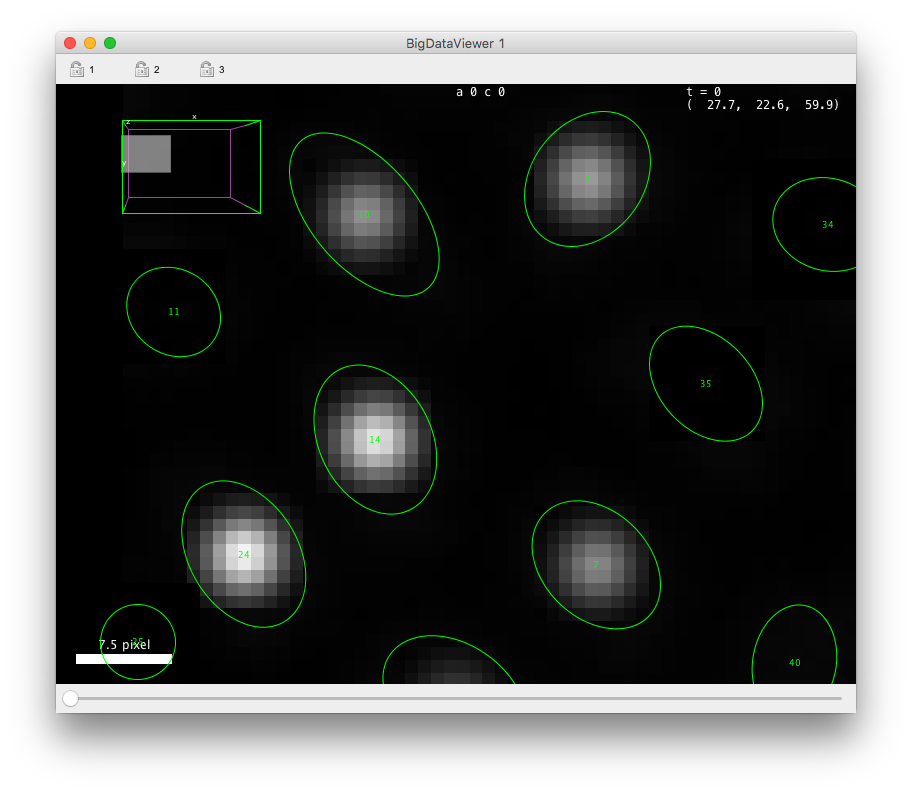
\includegraphics[width=6cm]{figures/Mastodon_GaussMeanIntensityWeights.png}
    \caption{Illustration of the Gaussian weights used in the \textbf{Spot gaussian-filtered intensity} feature.}
    \label{fig:SpotGaussWeights}
\end{figure}
    
\subsubsection{Spot median intensity.}

There is one projection of this feature per channel.
It reports the median intensity in the center of the spot for each channel.
The median is calculated inside a box that fits in the smallest radius of the ellipsoid.
The Figure~\ref{fig:SpotMedianBox} illustrates what this box looks like for several spots.

\begin{figure}
    \centering
    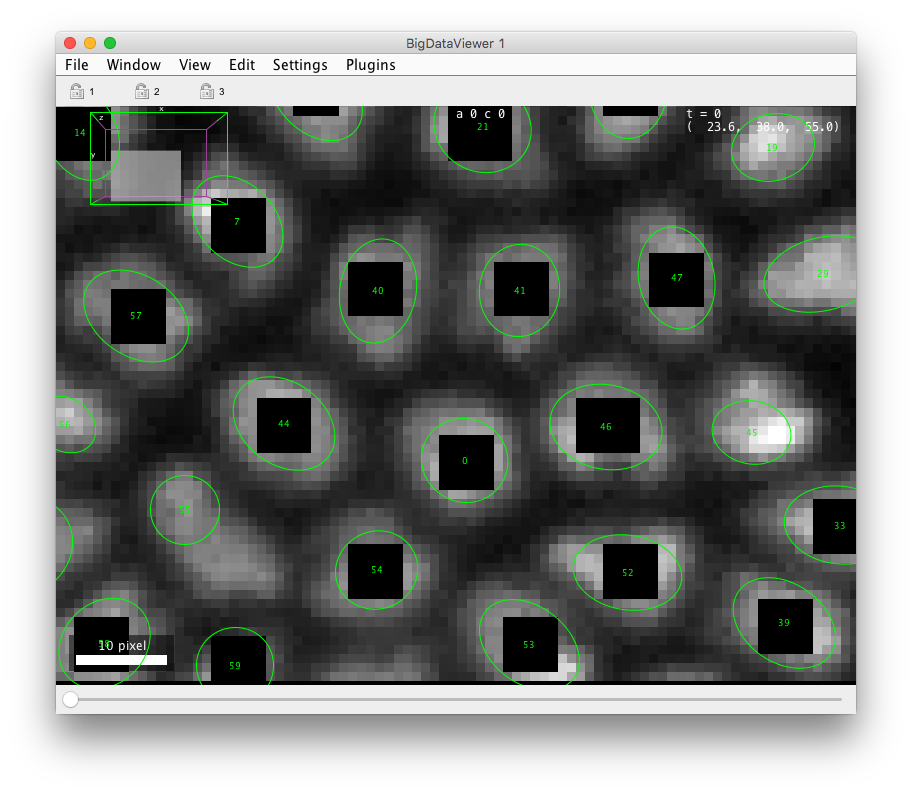
\includegraphics[width=6cm]{figures/Mastodon_Median-feature-pixels.png}
    \caption{Illustration of the box in which the \textbf{Spot median intensity} feature is calculated.}
    \label{fig:SpotMedianBox}
\end{figure}

\subsubsection{Other spot features.}
{
\footnotesize

\begin{tabular}{p{0.17\textwidth}|p{0.17\textwidth}|p{0.57\textwidth}}

    \toprule
    \textbf{Feature name} &
    \textbf{Projections} &
    \textbf{Description}             
    \\ \midrule
    
    \multicolumn{2}{l|}{Spot frame} & 
    The spot frame.
    \\ \midrule

    \multicolumn{2}{l|}{Spot N links} & 
    The total number of links, incoming and outgoing, of the spot.
    \\ \midrule
    
    Spot position &
    X, Y, Z &
    The spot center position, in physical units.
    \\ \midrule
    
    \multicolumn{2}{l|}{Spot radius} & 
    The spot radius in physical units. 
    
    For spots that are ellipsoids, returns a radius using the geometric mean of the spot ellipsoid radiuses. This approximation is such that the sphere with the reported radius and the spot ellipsoid have the same volume.
    \\ \midrule
    
    Spot sum intensity & 
    One value per channel &
    The total spot intensity for all the pixels inside the spot ellipsoid.
    \\ \midrule
    
    \multicolumn{2}{l|}{Spot track ID} &
    The ID of the track the spot belongs to.
    Track IDs are positive integer numbers starting from 0.
    \\ \midrule

\end{tabular}
}

\subsection{Link features.}

\subsection{Track features.}